\renewcommand{\chaptername}{Chapter} 
\chapter{Reanalysis of psychophysical biomarkers}\label{chap8}
The main objective of GLM-HMM modelization was to apply a probabilistic model to detect hidden states in participants' responses. The GLM-HMM model provided a structured approach for estimating posterior state probabilities on a trial-by-trial basis and constructing a transition matrix, which allowed us to analyze the likelihood of participants remaining in or transitioning between states. Unlike traditional signal detection theory tasks, where a ground truth exists and ROC curves can be used to assess performance, our challenge was the absence of a correct response in the reverse correlation experiment. This made it impossible to directly determine how many states participants could switch between. To overcome this, we conducted extensive simulations with known true states, enabling us to optimize model fitting using maximum a posteriori (MAP) estimation by selecting the most appropriate priors.\newline
Applying these optimized priors led to several unexpected findings. Most notably, patients showed a stronger tendency to remain in the perseverative state, making significantly fewer transitions back to an engaged, stimulus-driven decision mode. This suggests that once patients enter a perseverative state, they struggle to re-engage with external sensory information, whereas controls demonstrate greater flexibility, dynamically adjusting their responses based on stimulus input.\newline
One of the key findings in Chapter 4 was that internal noise, rather than just internal representation, plays a major role in differentiating patients from controls. However, we recognized that internal noise estimates from the double-pass method were contaminated by perseveration in patients, leading to inflated values. Thus, a primary goal in this chapter was to assess whether removing perseverative trials would reduce internal noise estimates. Our results confirmed this hypothesis: after filtering out perseverative trials, internal noise values—previously estimated through the confidence interval of the GLM—decreased significantly, supporting the idea that perseveration artificially inflates internal noise measurements in patients.\newline
These findings highlight the importance of distinguishing true internal noise from noise introduced by behavioral biases, reinforcing the need for probabilistic models like GLM-HMM to uncover underlying cognitive states rather than relying solely on traditional psychophysical measures.

\section{Qualitative impact of new methodologies on Kernel typicality}

In Chapter \ref{chap3}, we introduced the linear models used to estimate kernels (internal representations through weighted sums and GLMs) in reverse correlation tasks. These models have been applied to various experimental paradigms. Later, in Chapter \ref{chap5}, we discussed the limiting factors affecting their performance.

Our primary objective was to detect perseverative trials and obtain a more accurate estimation of the GLM kernel for engaged trials. However, as discussed in the previous chapter, simply removing perseverative trials does not necessarily improve the similarity of kernel typicality between perseverative patients and controls, figure \ref{fig:kernels_segments_methods} and \ref{fig:kernels_comparisons} showing that after removing perseverative trials, the estimated kernel magnitudes tend to be lower. One possible explanation is that a significant proportion of patient responses occur in the perseverative state. Specifically, while controls have an average of 119 engaged trials out of 150 (80\%), patients have significantly fewer, with only 62 engaged trials out of 150 (41\%).

This substantial reduction in trial count affects kernel estimation, as a reliable estimation requires at least 200 trials (as demonstrated in Figure \ref{fig:experiment}). Consequently, the loss of trials in perseverative patients limits our ability to obtain robust kernel estimates, highlighting the challenge of accurately characterizing their internal representations, as already been shown by the simulation validation in chapter \ref{chap7}.

\begin{figure}[H]
    \centering
    \includegraphics[width=17cm,height=7cm]{MainLayout/Images/chapter8/kernels_segments_methods.jpg}
    \caption{Main Title for First Image \\ \small Subtitle for the first graphic.}
    \label{fig:kernels_segments_methods}
\end{figure}

\begin{figure}[H]
    \centering
    
\includegraphics[width=17cm,height=7cm]{MainLayout/Images/chapter8/kernel_comparison_methods.jpg}
    \caption{Main Title for First Image \\ \small Subtitle for the first graphic.}
    \label{fig:kernel_comparison_methods}
\end{figure}
\begin{figure}[H]
    \centering
    
\includegraphics[width=17cm,height=7cm]{MainLayout/Images/chapter8/kernel_comparison_types_methods.jpg}
    \caption{Main Title for First Image \\ \small Subtitle for the first graphic.}
    \label{fig:kernel_comparison_methods}
\end{figure}
\section{Qualitative impact of new methodologies on Internal noise}
\begin{figure}[H]
    \centering
    
\includegraphics[width=17cm,height=7cm]{MainLayout/Images/chapter8/internal_noise_comparison_types_glms.jpg}
    \caption{Main Title for First Image \\ \small Subtitle for the first graphic.}
    \label{fig:internal_noise_comparison_types_glms}
\end{figure}
\begin{figure}[H]
    \centering
    
\includegraphics[width=17cm,height=7cm]{MainLayout/Images/chapter8/internal_noise_comparison_glms.jpg}
    \caption{Main Title for First Image \\ \small Subtitle for the first graphic.}
    \label{fig:internal_noise_comparison_glms}
\end{figure}
\begin{figure}[H]
    \centering
    
\includegraphics[width=17cm,height=7cm]{MainLayout/Images/chapter8/internal_noise_comparison_types_glms.jpg}
    \caption{Main Title for First Image \\ \small Subtitle for the first graphic.}
    \label{fig:internal_noise_comparison_types_glms}
\end{figure}
\section{Probability of transition to perseveration as a new biomarker} 
\begin{figure}[H]
    \centering
    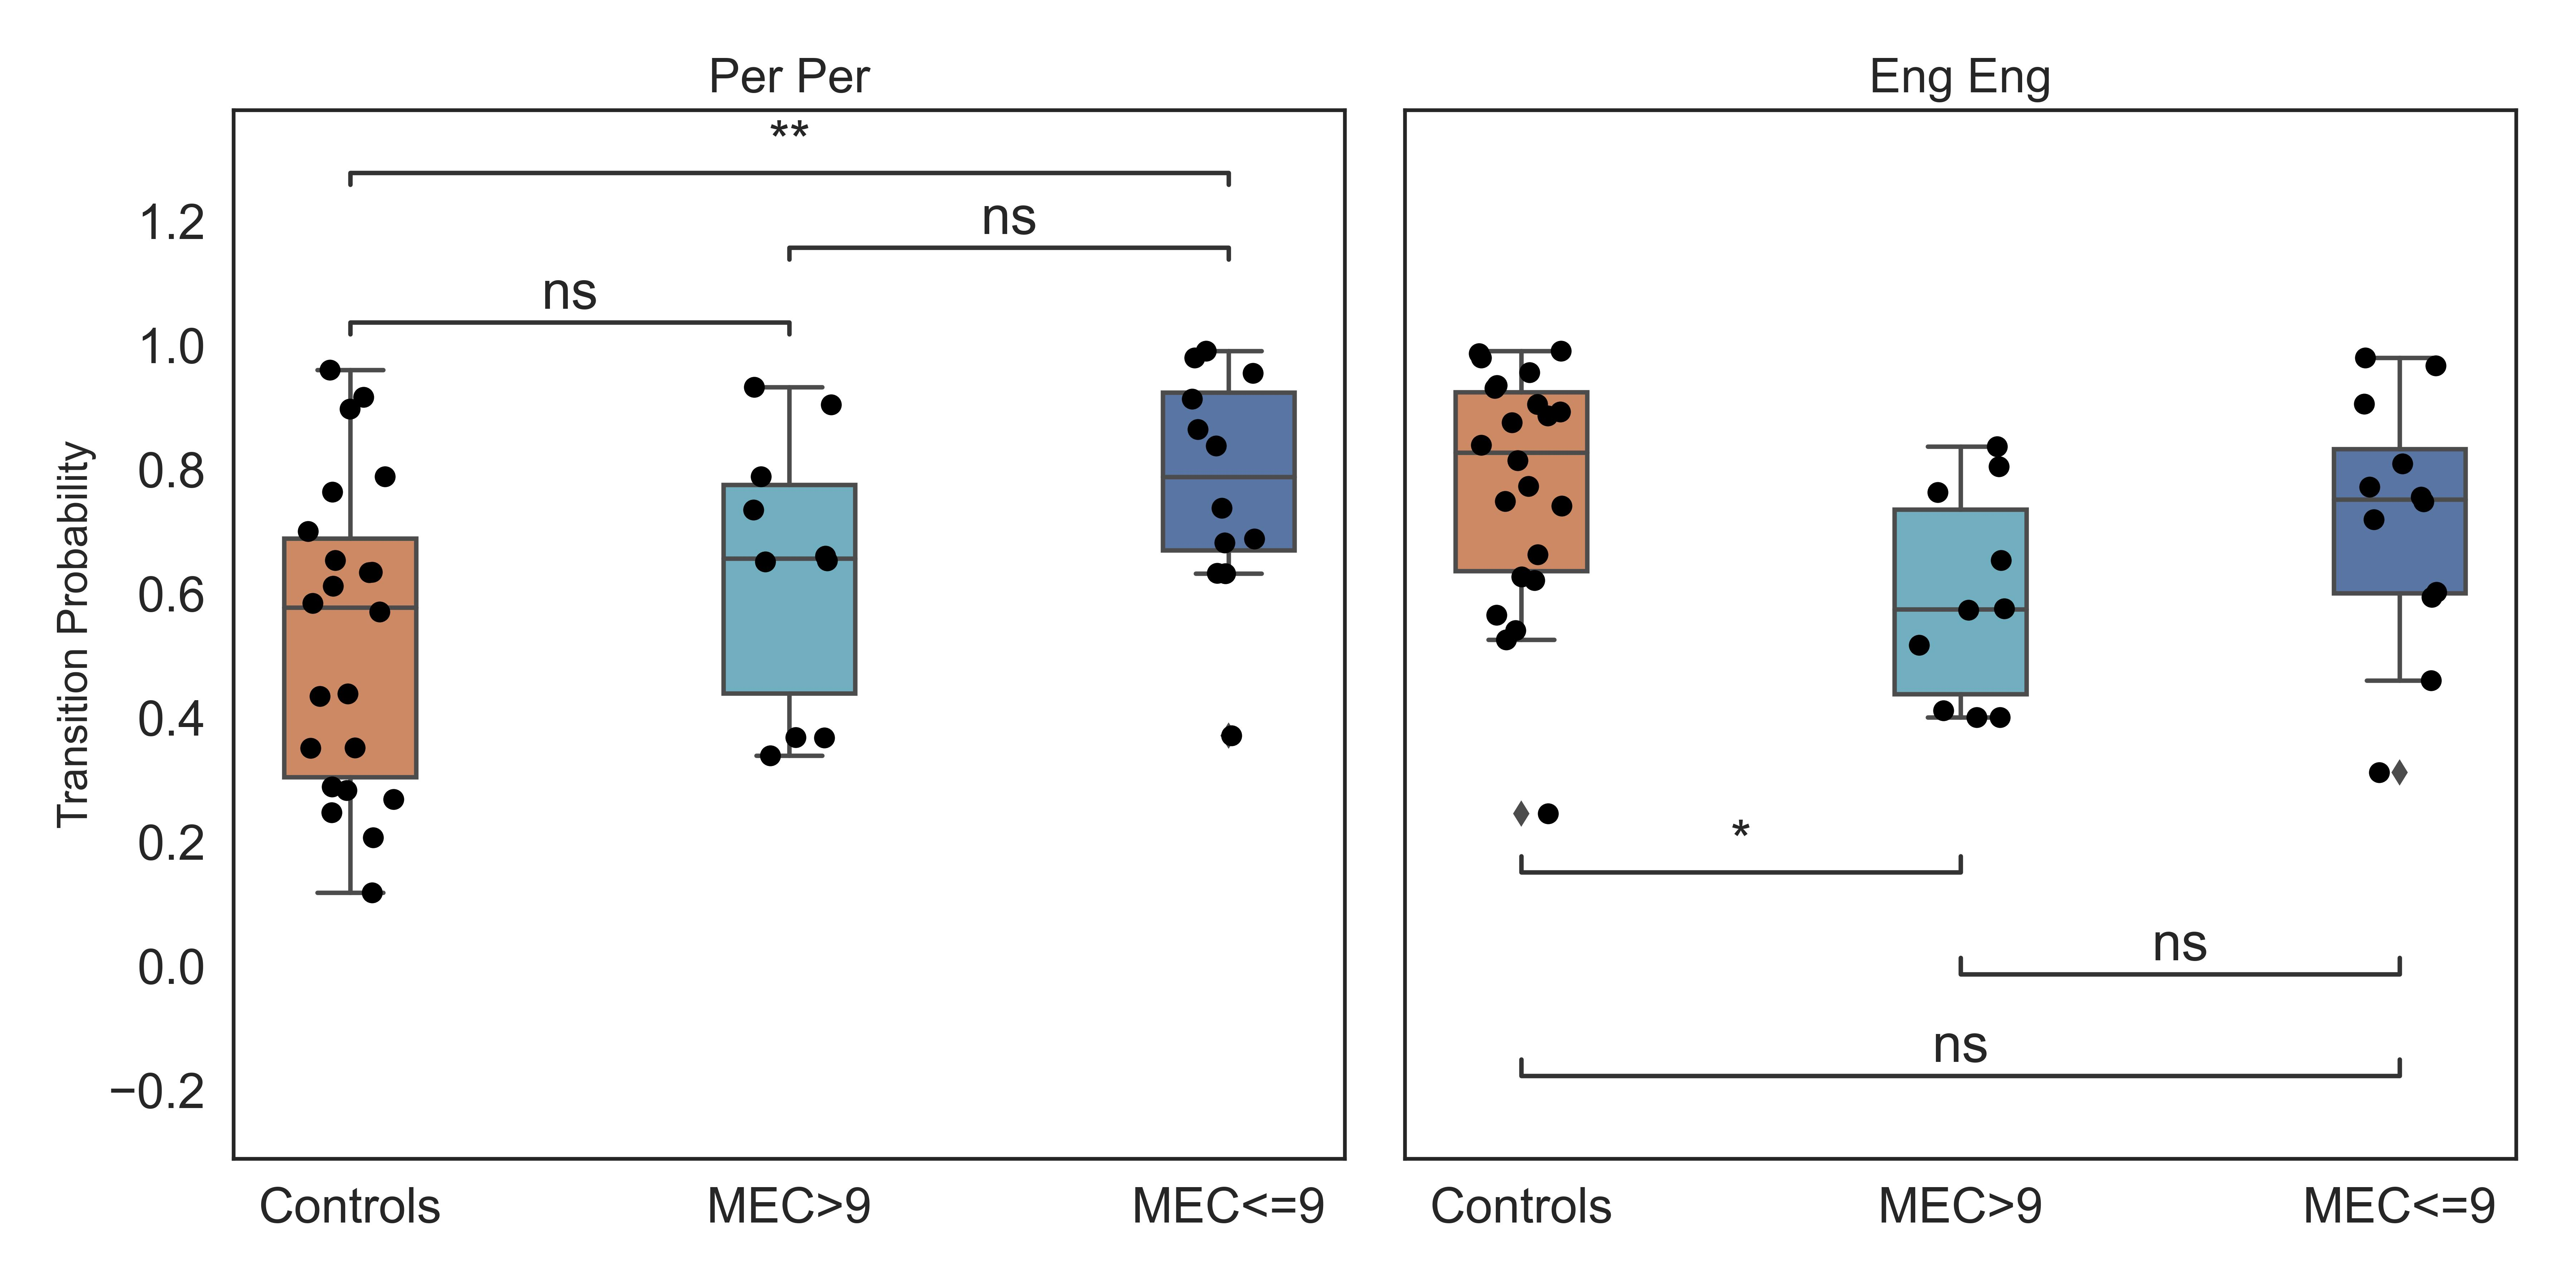
\includegraphics[width=17cm,height=7cm]{MainLayout/Images/chapter8/sticky_state.jpg}
    \caption{Main Title for First Image \\ \small Subtitle for the first graphic.}
    \label{fig:sticky_state}
\end{figure}
\begin{figure}[H]
    \centering
    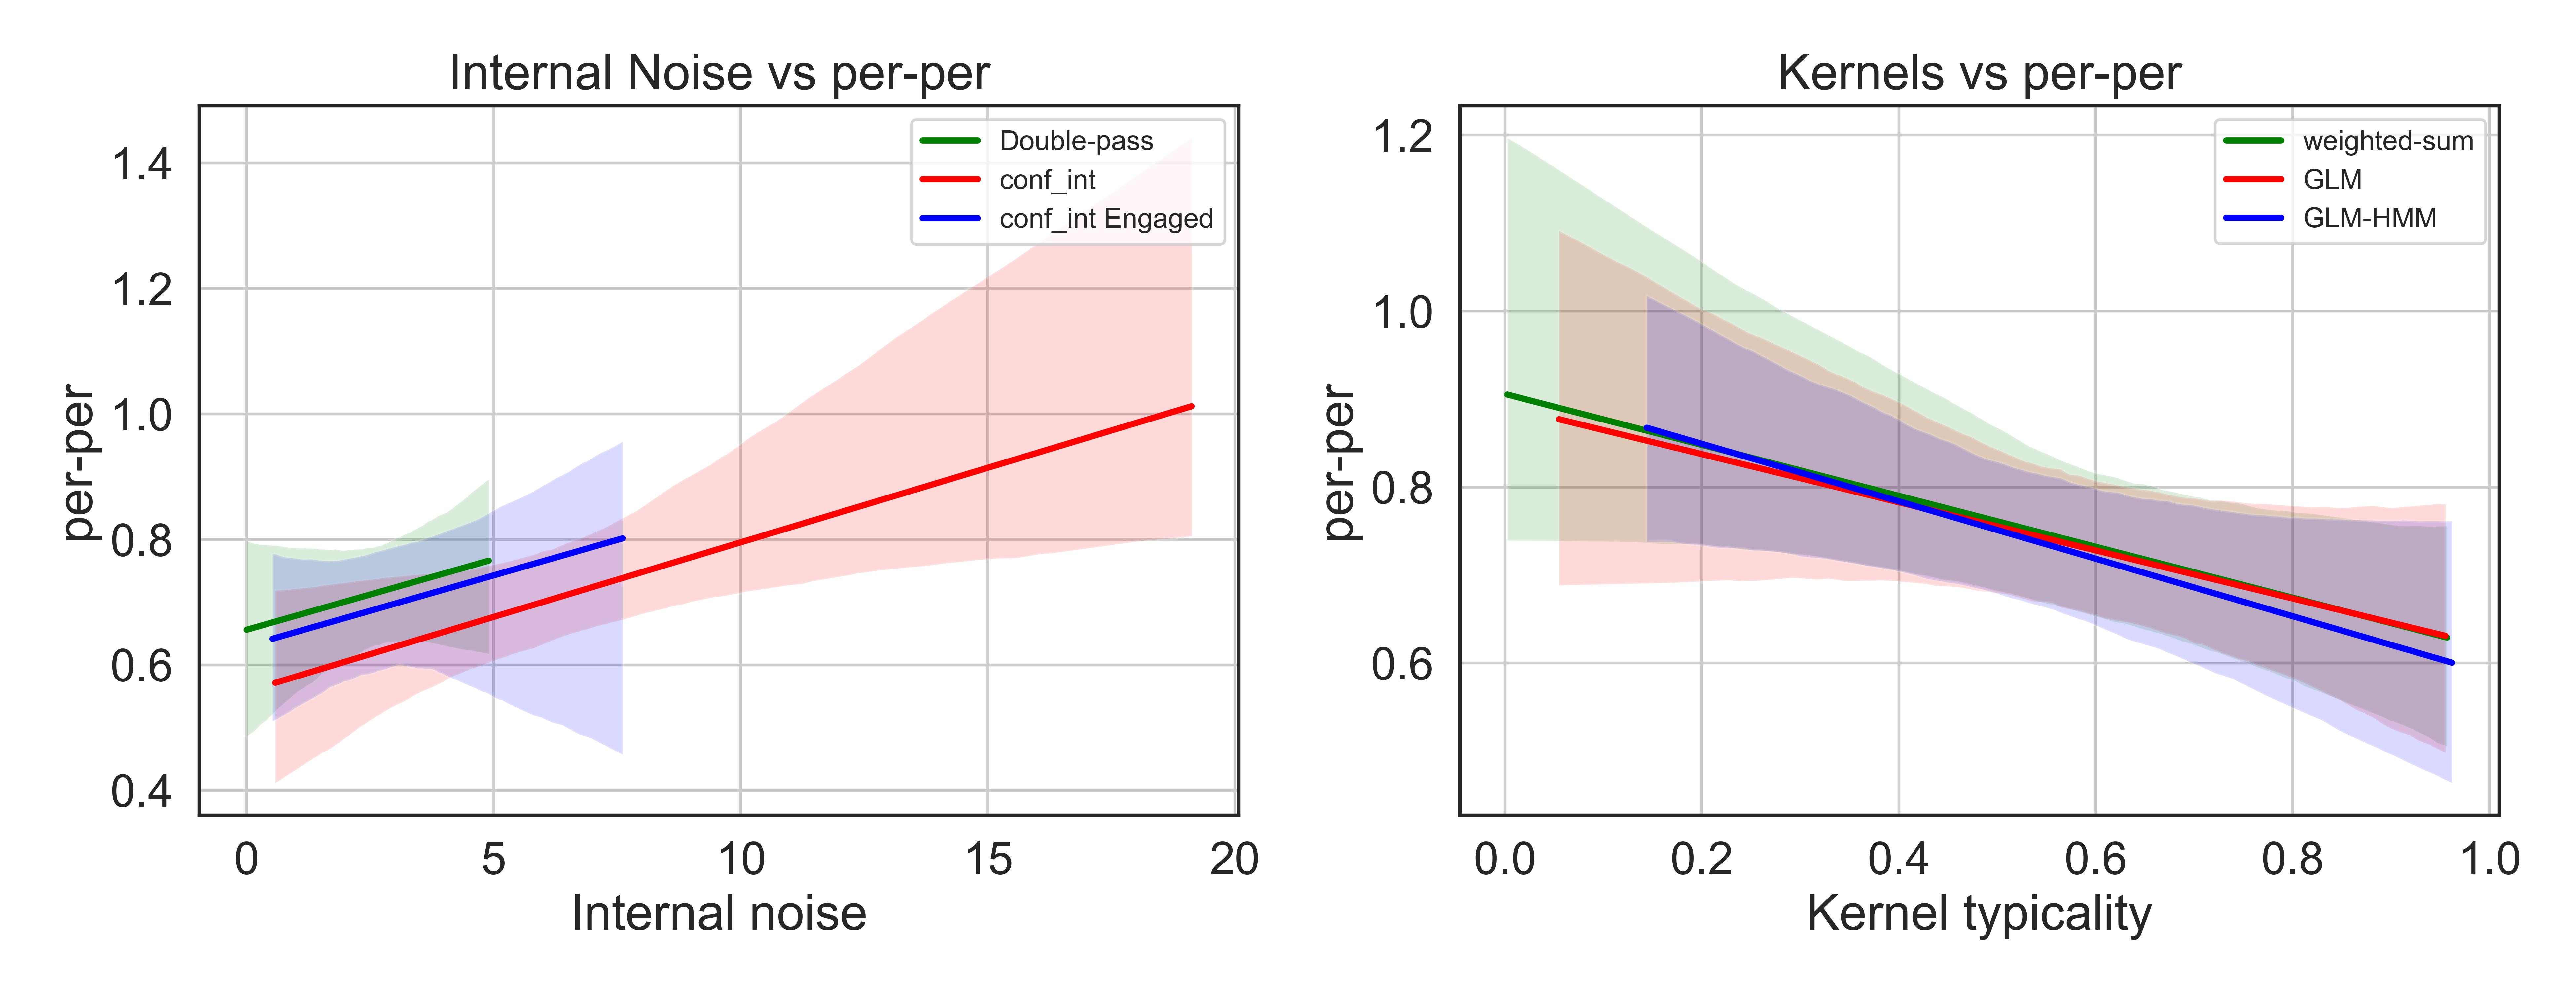
\includegraphics[width=17cm,height=7cm]{MainLayout/Images/chapter8/regression_results_per_per.jpg}
    \caption{Main Title for First Image \\ \small Subtitle for the first graphic.}
    \label{fig:regression_results_per_per}
\end{figure}
\begin{figure}[H]
    \centering
    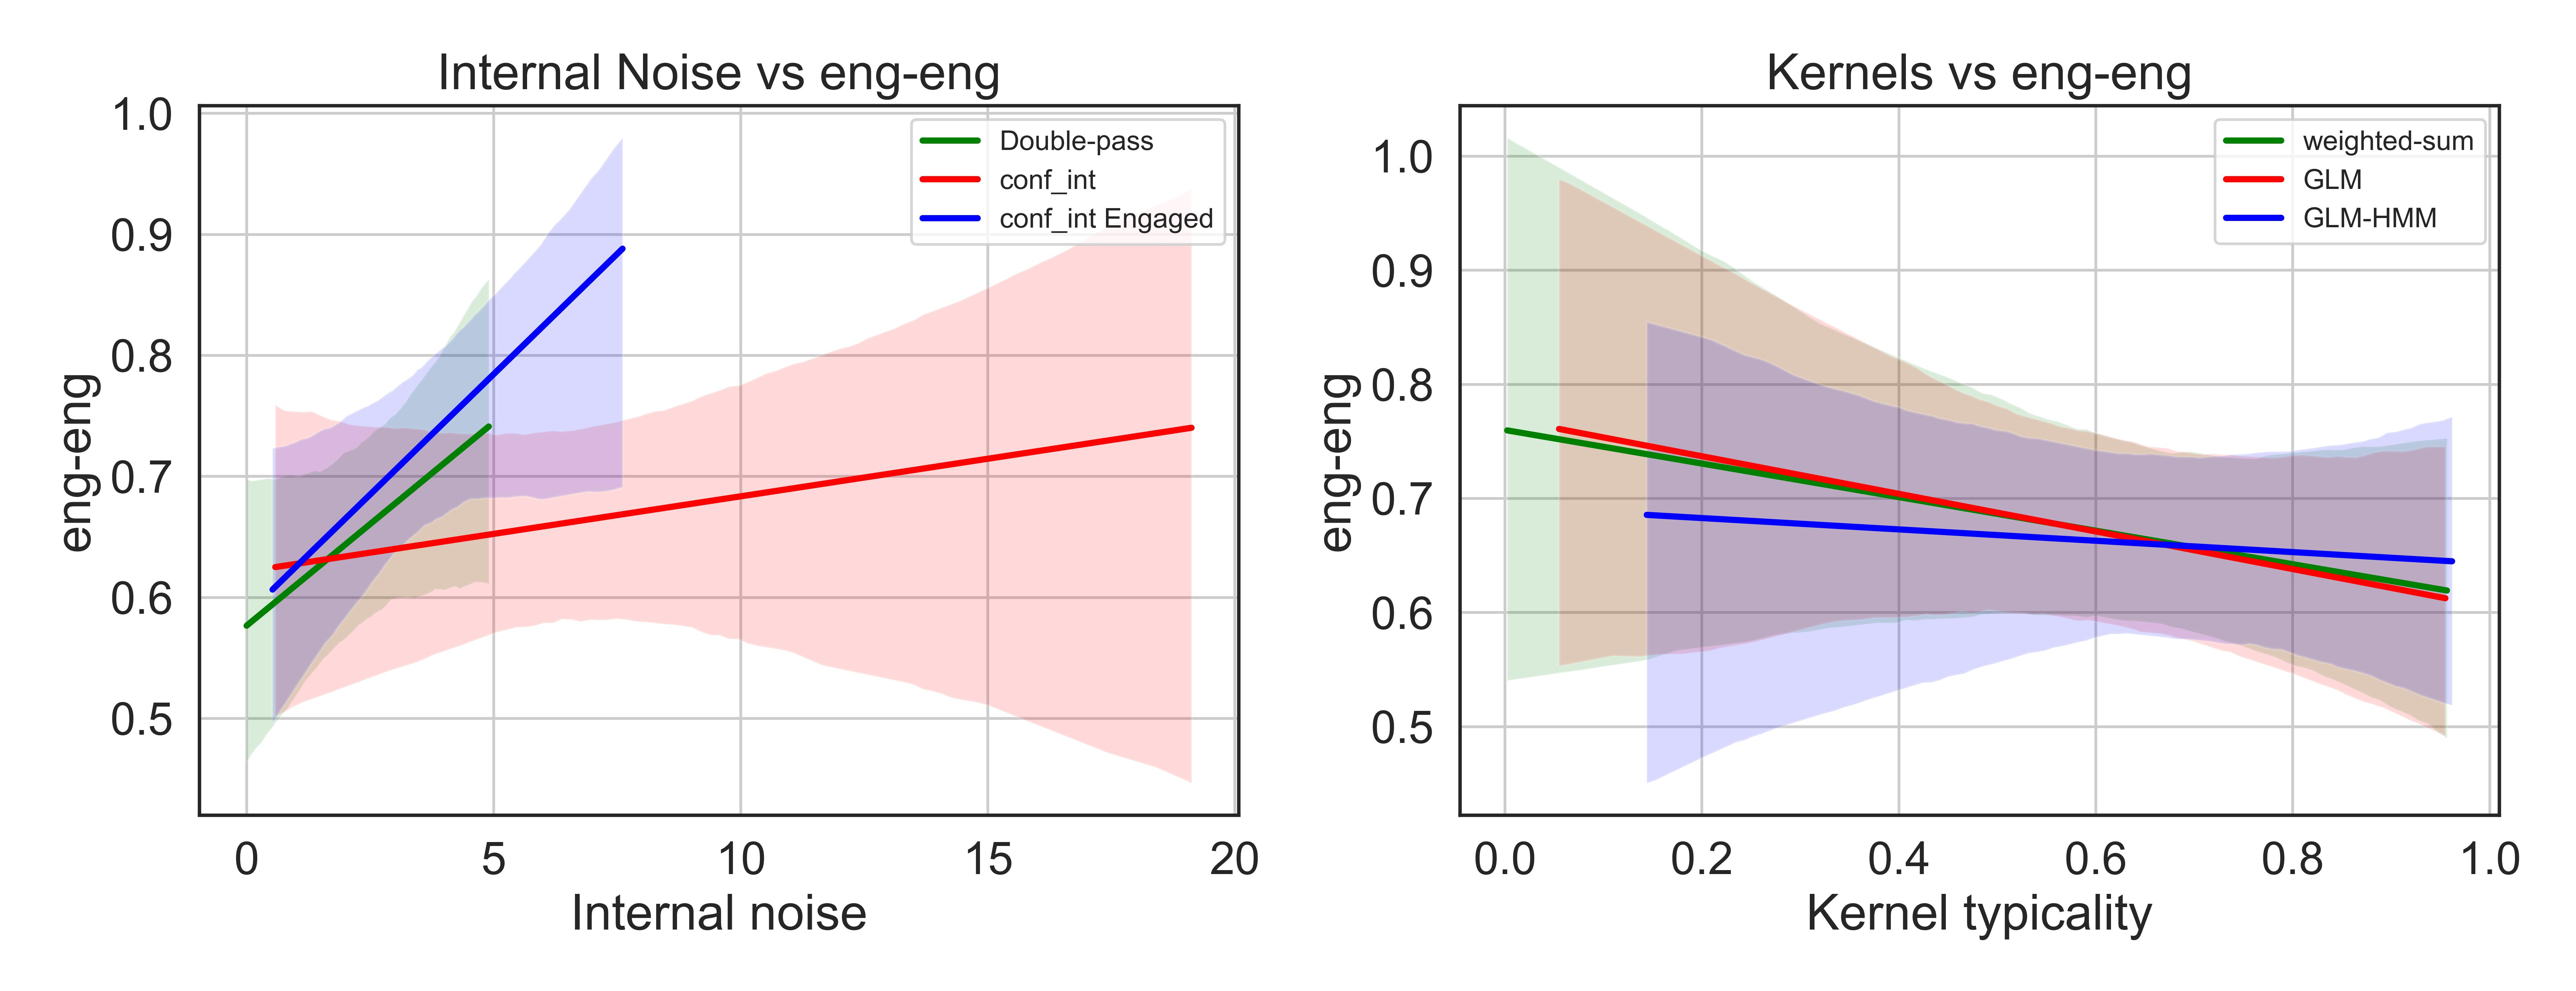
\includegraphics[width=17cm,height=7cm]{MainLayout/Images/chapter8/regression_results_eng_eng.jpg}
    \caption{Main Title for First Image \\ \small Subtitle for the first graphic.}
    \label{fig:regression_results_eng_eng}
\end{figure}

\section{Quantitative impact on old analysis}

\subsection {Correlation with MEC} 
\begin{figure}[H]
    \centering
    
\includegraphics[width=17cm,height=7cm]{MainLayout/Images/chapter8/regression_results_mec.jpg}
    \caption{Main Title for First Image \\ \small Subtitle for the first graphic.}
    \label{fig:regression_results_mec}
\end{figure}

\begin{figure}[H]
    \centering
    
\includegraphics[width=17cm,height=7cm]{MainLayout/Images/chapter8/regression_results_mec_c.jpg}
    \caption{Main Title for First Image \\ \small Subtitle for the first graphic.}
    \label{fig:regression_results_mec_c}
\end{figure}

\begin{figure}[H]
    \centering
    
\includegraphics[width=17cm,height=7cm]{MainLayout/Images/chapter8/regression_results_mec_r.jpg}
    \caption{Main Title for First Image \\ \small Subtitle for the first graphic.}
    \label{fig:regression_results_mec_r}
\end{figure}

\subsection {Correlation with Airtac} 
\begin{figure}[H]
    \centering
    
\includegraphics[width=17cm,height=7cm]{MainLayout/Images/chapter8/regression_results_airtac.jpg}
    \caption{Main Title for First Image \\ \small Subtitle for the first graphic.}
    \label{fig:regression_results_airtac}
\end{figure}

\begin{figure}[H]
    \centering
    
\includegraphics[width=17cm,height=7cm]{MainLayout/Images/chapter8/regression_results_airtac_dur_discr.jpg}
    \caption{Main Title for First Image \\ \small Subtitle for the first graphic.}
    \label{fig:regression_results_airtac_dur_discr}
\end{figure}

\begin{figure}[H]
    \centering
    
\includegraphics[width=17cm,height=7cm]{MainLayout/Images/chapter8/regression_results_airtac_int_discr.jpg}
    \caption{Main Title for First Image \\ \small Subtitle for the first graphic.}
    \label{fig:regression_results_airtac_int_discr}
\end{figure}
\subsection {Correlation with other clinical measures} 
\begin{figure}[H]
    \centering
    
\includegraphics[width=17cm,height=7cm]{MainLayout/Images/chapter8/regression_results_lama_prec.jpg}
    \caption{Main Title for First Image \\ \small Subtitle for the first graphic.}
    \label{fig:regression_results_lama_prec}
\end{figure}
\begin{figure}[H]
    \centering
    
\includegraphics[width=17cm,height=7cm]{MainLayout/Images/chapter8/regression_results_mbea_total.jpg}
    \caption{Main Title for First Image \\ \small Subtitle for the first graphic.}
    \label{fig:regression_results_mbea_total}
\end{figure}

\begin{figure}[H]
    \centering
    
\includegraphics[width=17cm,height=7cm]{MainLayout/Images/chapter8/regression_results_hads.jpg}
    \caption{Main Title for First Image \\ \small Subtitle for the first graphic.}
    \label{fig:regression_results_hads}
\end{figure}
\section{Discussion of the differences} 
\begin{figure}[H]
    \centering
    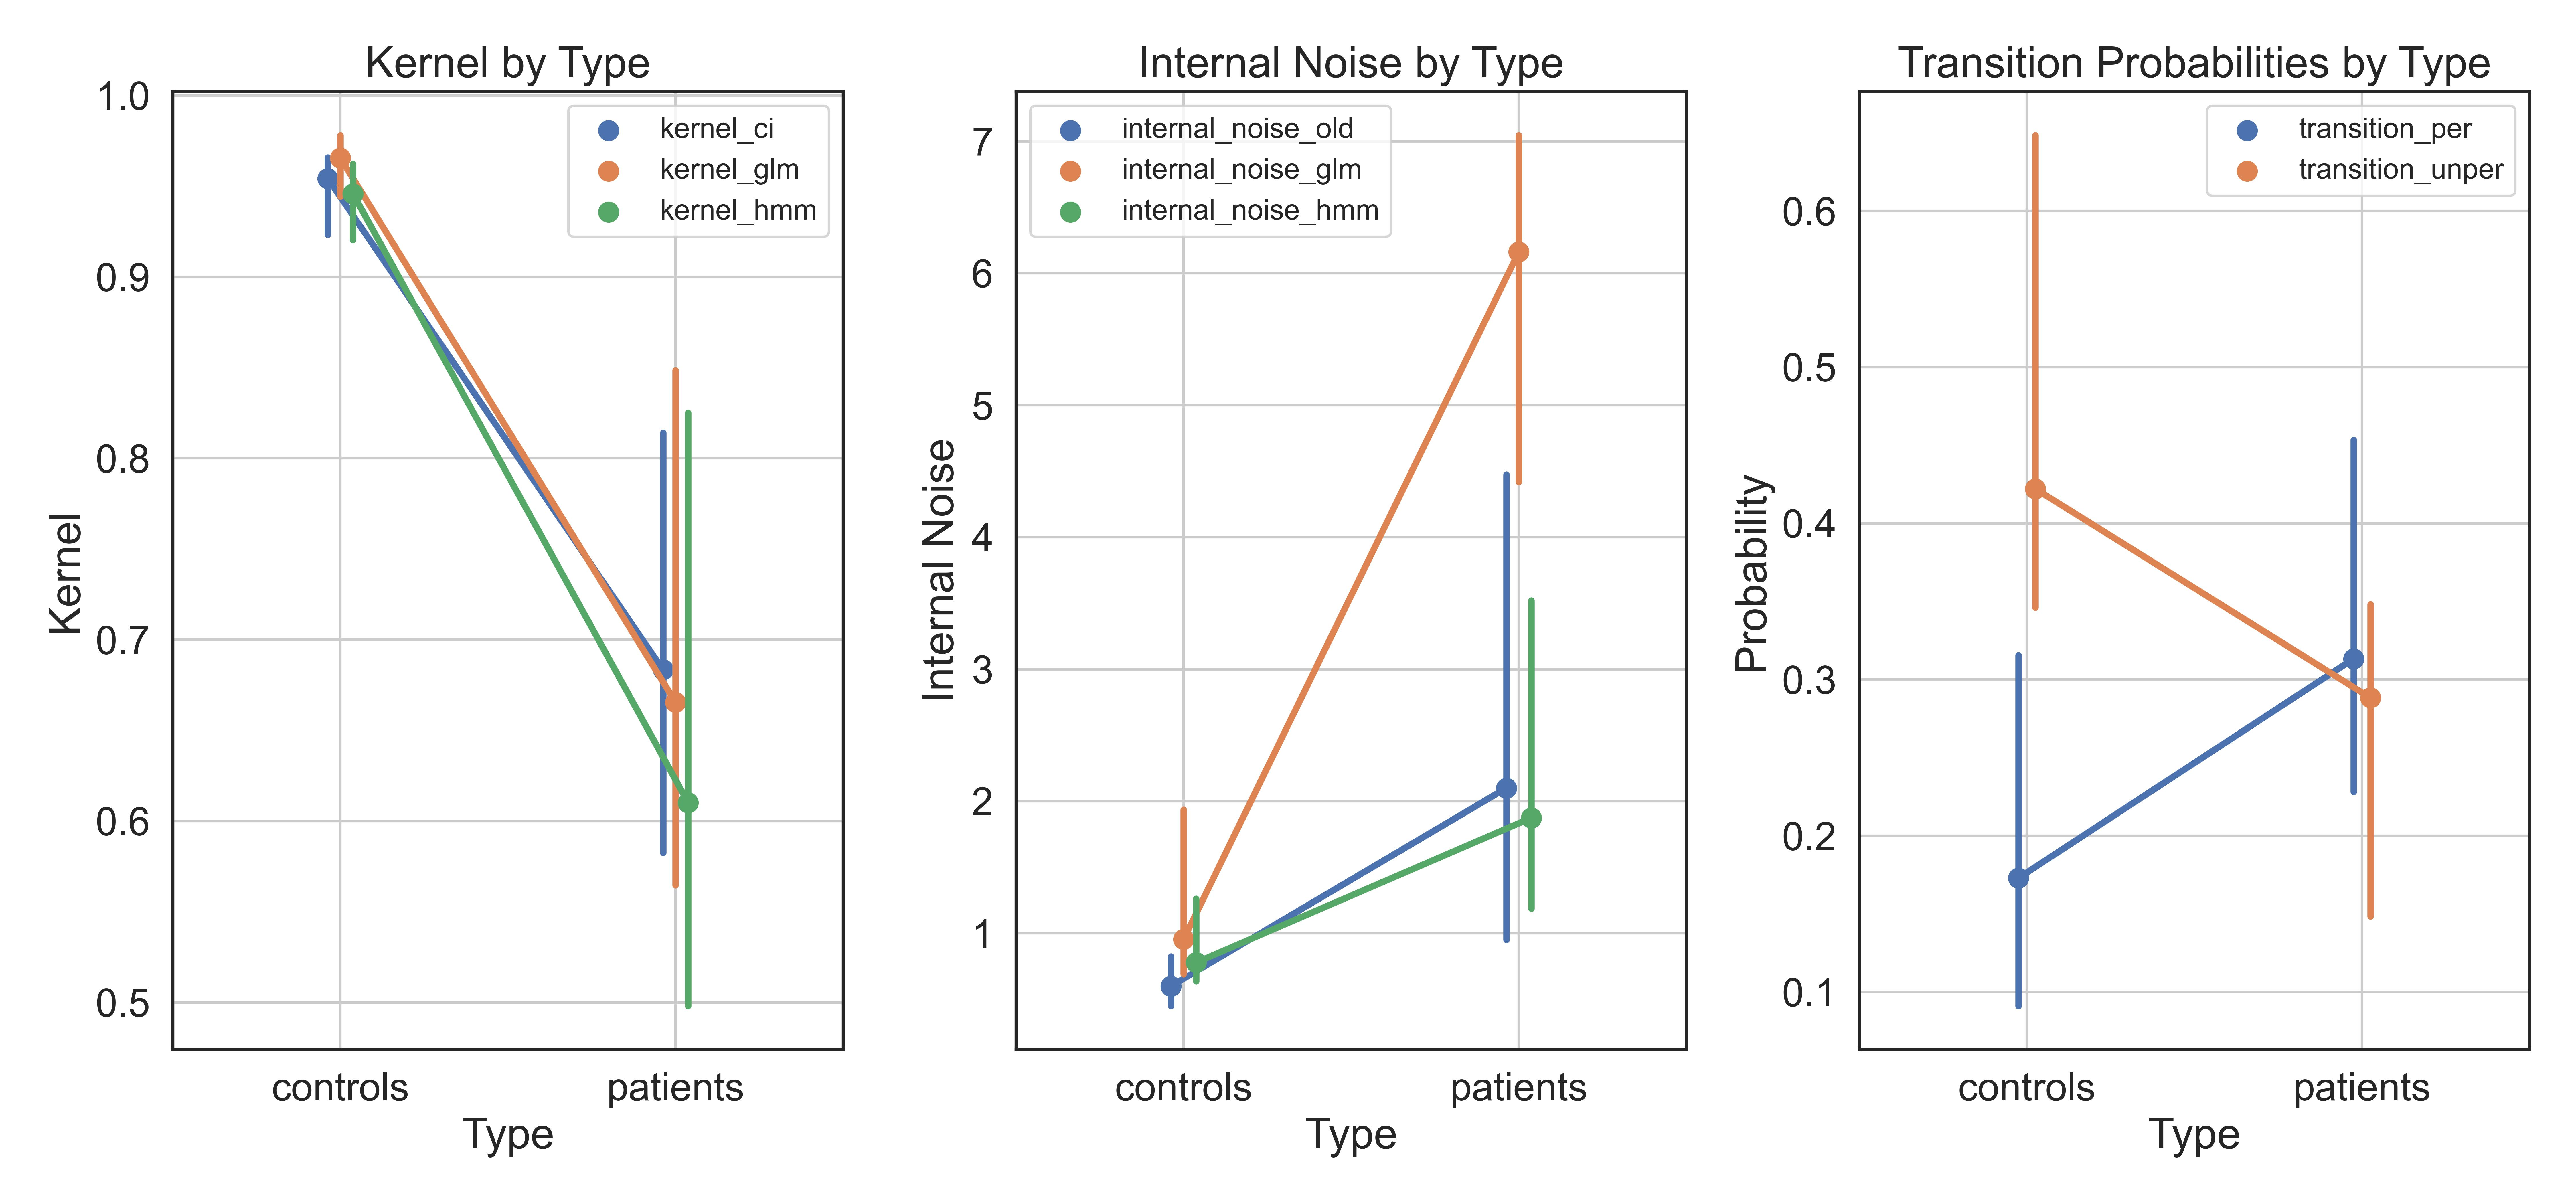
\includegraphics[width=17cm,height=7cm]{MainLayout/Images/chapter8/revcor_measures.jpg}
    \caption{Main Title for First Image \\ \small Subtitle for the first graphic.}
    \label{fig:revcor_measures}
\end{figure}

\begin{figure}[H]
    \centering
    \includegraphics[width=17cm,height=7cm]{MainLayout/Images/chapter8/kernels_segments_subjects_controls.jpg}
    \caption{Main Title for First Image \\ \small Subtitle for the first graphic.}
    \label{fig:kernels_segments_subjects_controls}
\end{figure}

\begin{figure}[H]
    \centering
    \includegraphics[width=17cm,height=7cm]{MainLayout/Images/chapter8/kernels_segments_subjects_patients.jpg}
    \caption{Main Title for First Image \\ \small Subtitle for the first graphic.}
    \label{fig:kernels_segments_subjects_patients}
\end{figure}